\section{Straight-Line Program}
\label{slpsec}
Nel contesto \textit{bioinformatico} una delle principali problematiche è la
gestione di testi molto estesi. Pensiamo, ad esempio, al caso umano. Il primo
cromosoma, il più lungo tra i cromosomi umani, conta circa $247.249.719$
\textit{bps} (paia di basi), nonostante, è bene segnalare, l'uomo
non sia affatto l'essere vivente con il genoma più esteso. Fatta questa breve
premessa, è facile comprendere l'importanza degli algoritmi e delle strutture
dati per la compressione di testi.\\
Per questa tesi si è quindi pensato all'uso dei cosiddetti \textbf{Straight-Line
  Programs (\textit{SLP})}. In termini 
generici, un \textit{SLP} è una \textbf{grammatica context-free} che 
genera una e una sola parola \cite{slpsurvey}, parlando, quindi, di
\textbf{grammar-based compression}.
\begin{definizione}
  Sia dato un alfabeto finito $\Sigma$ di simboli terminali. Sia data una
  stringa $s=a_1,a_2,\ldots, a_n\in\Sigma^{*}$, lunga $n$ e costruita
  sull'alfabeto $\Sigma$, avendo $a_i\in\Sigma$, $\forall\, i \mbox{
    t.c. }1\leq i\leq n$. Si denota, con $alph(s)=\{a_1,a_2,\ldots
  a_n\}$, l'insieme dei simboli della stringa $s$.\\
  Si definisce \textbf{SLP}, costruito sull'alfabeto $\Sigma$, una grammatica
  context-free $\mathcal{A}$ tale che: 
  \begin{equation}
    \label{eq:slpdef}
    \mathcal{A}=\left(\mathcal{V}, \Sigma, \mathcal{S}, \mathcal{P}\right)
  \end{equation}
  Dove:
  \begin{itemize}
    \item $\mathcal{V}$ è l'insieme dei simboli non terminali
    \item $\Sigma$ è l'insieme dei simboli terminali
    \item $\mathcal{S}\in \mathcal{V}$ è il simbolo iniziale non terminale
    \item $\mathcal{P}$ è l'insieme delle produzioni, avendo che:
    \begin{equation}
      \label{eq:slpprod}
      \mathcal{P}\subseteq \mathcal{V}\times\left(\mathcal{V}\cup
        \Sigma\right)^{*}
    \end{equation}
  \end{itemize}
  Tale grammatica, per essere un \textit{SLP}, deve soddisfare due proprietà:
  \begin{enumerate}
    \item si ha una e una sola produzione $(A,\alpha)\in \mathcal{P}$,
    $\forall\, A\in \mathcal{V}$ e con $\alpha\in
    \left(\mathcal{V}\cup\Sigma\right)^{*}$ (si 
    noti che la produzione $(A,\alpha)$ può anche essere indicata con
    $A\to\alpha$) 
    \item la relazione $\{(A,B)\,|\,\,(A,\alpha)\in\mathcal{P},\,\,B\in
    alph(\alpha)\}$ è aciclica
    \dc{verificare questo secondo punto}
  \end{enumerate}
  Si ha quindi che la grandezza dell'SLP è calcolabile come:
  \begin{equation}
    \label{eq:slplen}
    |\mathcal{A}| = \sum_{(A,\alpha)\in\mathcal{P}}|\alpha|
  \end{equation}
  Il linguaggio $\mathcal{A}$ generato da un \textit{SLP}
  consiste in una singola parola, denotata da $eval(\mathcal{A})$.
\end{definizione}
A partire dall'\textit{SLP} $\mathcal{A}$ si genera un \textbf{albero
  di derivazione}, che, nel dettaglio, è un \textit{albero radicato e ordinato}
dove la \textit{radice} è etichettata con $\mathcal{S}$, ogni \textit{nodo
  interno} è etichettato con un simbolo di $\mathcal{V}\cup\Sigma$ e ogni foglia
è etichettata con un simbolo di $\Sigma$.
\begin{esempio}
  \label{ese:slpgagie}
  Si prenda, ad esempio \cite{slpgagie}, la seguente stringa:
  \[s=\mbox{GATTAGATACAT}\,\$\mbox{GATTACATAGAT}\]
  Si potrebbe produrre il seguente \emph{SLP}:
  \begin{multicols}{2}
    \begin{itemize}
      \item $\mbox{S}\to \mbox{ZWAY}\,\$\mbox{ZYAW}$
      \item $\mbox{Z}\to \mbox{WX}$
      \item $\mbox{Y}\to \mbox{CV}$
      \item $\mbox{X}\to \mbox{TA}$
      \item $\mbox{W}\to \mbox{GV}$
      \item $\mbox{V}\to \mbox{AT}$
    \end{itemize}
  \end{multicols}
  Al quale corrisponde il seguente \emph{albero di derivazione}:
  \begin{figure}[H]
    \centering
    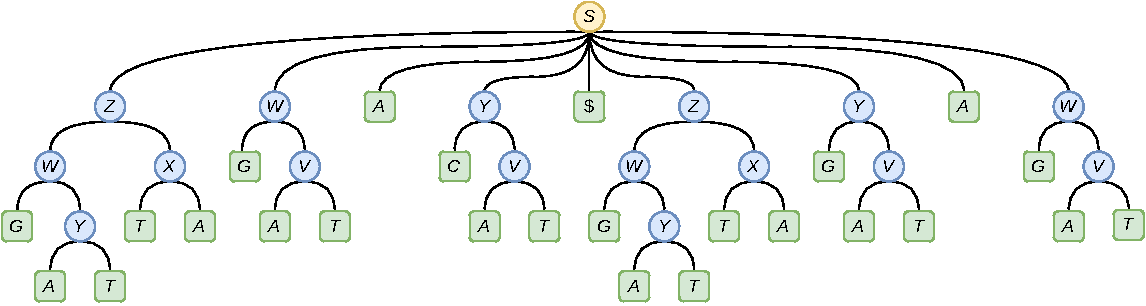
\includegraphics[width=\textwidth]{img/slpgagie.pdf}
  \end{figure}
  Si noti che il simbolo
  iniziale non terminante, ovvero la radice, è indicata con un cerchio giallo, i
  simboli non terminanti, ovvero i nodi interni, sono indicati dai cerchi blu
  mentre i simboli terminanti, ovvero le foglie, sono indicati dai quadrati
  verdi.
\end{esempio}
Nel 2020, Gagie et al. \cite{slpgagie} 
proposero un articolo, a cui si rimanda per approfondimenti, in merito a
miglioramenti prestazionali per il \textit{random access} all'\textit{SLP},
anche tramite l'uso dei \textit{bitvector sparsi}.\\
Si stima che il tempo necessario al
\textit{random access} su un testo $T$ compresso tramite
\textit{SLP}, sia in tempo:
\begin{equation}
  \label{eq:slptime}
  \mathcal{O}\left(\log (eval(\mathcal{A}))\right)
\end{equation}
L'uso di tale variante degli \textit{SLP} è stato cruciale, come si vedrà più
avanti in questa tesi, per la costruzione della versione run-length encoded sia
della \textbf{Burrows-Wheeler Transform (\textit{BWT})} che della
\textbf{Positional Burrows-Wheeler Transform (\textit{PBWT})}.
\subsection{Longest Common Extension}
Oltre a permettere \textit{random access} alla testo compresso, 
l'uso degli \textit{SLP} permette di effettuare 
un'altra operazione in modo efficiente: le \textbf{Longest Common Extension
  (\textit{LCE}) queries}.
\begin{definizione}
  Dato un testo $T$, tale che $|T|=n$, il risultato della \textbf{LCE query} tra
  due posizioni $i$ e $j$, tali che $0\leq i,j<n$, corrisponde al più lungo
  prefisso comune tra le sotto-stringhe che hanno come indice di partenza $i$ e
  $j$, avendo quindi il più lungo prefisso comune tra $T[i,n-1]$ e $T[j,n-1]$.
\end{definizione}
Sfruttando l'\textit{SLP} del testo $T$ è quindi possibile effettuare due
\textit{random access} al testo compresso, in $i$ e $j$, per poi ``risalire''
l'albero al fine di computare il prefisso comune tra le due sottostringhe.\\
Si stima che il calcolo di una \textit{LCE query} sia effettuabile in tempo:
\begin{equation}
  \label{eq:lcetime}
  \mathcal{O}\left(\log (eval(\mathcal{A}))\right)
\end{equation}
I due concetti di \textit{SLP} e \textit{LCE query} verranno generalizzati, in
questa tesi, all'uso su matrici permettendo una rappresentazione compatta in
memoria, con \textit{random access}, per un pannello di aplotipi.
\dc{capire se sono necessari altri approfondimenti}